%%%%%%%%%%%%%%%%%%%%%%%%%%%%%%%%%%%%%%%%%%%%%%%%%%%%%%%%%%%%%%%%%%%%
%%%%%%%%%%%%%%%%%%%%%%%%%%%%%%%%%%%%%%%%%%%%%%%%%%%%%%%%%%%%%%%%%%%%
%%                                                                %%
%% An example for writting your thesis using LaTeX                %%
%% Original version by Luis Costa,  changes by Perttu Puska       %%
%% Support for Swedish added 15092014                             %%
%%                                                                %%
%% This example consists of the files                             %%
%%         thesistemplate.tex (versio 2.01)                       %%
%%         opinnaytepohja.tex (versio 2.01) (for text in Finnish) %%
%%         aaltothesis.cls (versio 2.01)                          %%
%%         kuva1.eps                                              %%
%%         kuva2.eps                                              %%
%%         kuva1.pdf                                              %%
%%         kuva2.pdf                                              %%
%%                                                                %%
%%                                                                %%
%% Typeset either with                                            %%
%% latex:                                                         %%
%%             $ latex opinnaytepohja                             %%
%%             $ latex opinnaytepohja                             %%
%%                                                                %%
%%   Result is the file opinnayte.dvi, which                      %%
%%   is converted to ps format as follows:                        %%
%%                                                                %%
%%             $ dvips opinnaytepohja -o                          %%
%%                                                                %%
%%   and then to pdf as follows:                                  %%
%%                                                                %%
%%             $ ps2pdf opinnaytepohja.ps                         %%
%%                                                                %%
%% Or                                                             %%
%% pdflatex:                                                      %%
%%             $ pdflatex opinnaytepohja                          %%
%%             $ pdflatex opinnaytepohja                          %%
%%                                                                %%
%%   Result is the file opinnaytepohja.pdf                        %%
%%                                                                %%
%% Explanatory comments in this example begin with                %%
%% the characters %%, and changes that the user can make          %%
%% with the character %                                           %%
%%                                                                %%
%%%%%%%%%%%%%%%%%%%%%%%%%%%%%%%%%%%%%%%%%%%%%%%%%%%%%%%%%%%%%%%%%%%%
%%%%%%%%%%%%%%%%%%%%%%%%%%%%%%%%%%%%%%%%%%%%%%%%%%%%%%%%%%%%%%%%%%%%

%% Uncomment one of these:
%% the 1st when using pdflatex, which directly typesets your document in
%% pdf (use jpg or pdf figures), or
%% the 2nd when producing a ps file (use eps figures, don't use ps figures!).
\documentclass[english,12pt,a4paper,pdftex,sci,utf8]{aaltothesis}
%\documentclass[english,12pt,a4paper,dvips]{aaltothesis}

%% To the \documentclass above
%% specify your school: arts, biz, chem, elec, eng, sci
%% specify the character encoding scheme used by your editor: utf8, latin1

\usepackage{graphicx}

%% Use this if you write hard core mathematics, these are usually needed
\usepackage{amsfonts,amssymb,amsbsy}

\usepackage{paralist}

%% Use the macros in this package to change how the hyperref package below 
%% typesets its hypertext -- hyperlink colour, font, etc. See the package
%% documentation. It also defines the \url macro, so use the package when 
%% not using the hyperref package.
%%
%\usepackage{url}

%% Use this if you want to get links and nice output. Works well with pdflatex.
\usepackage{hyperref}
\hypersetup{pdfpagemode=UseNone, pdfstartview=FitH,
  colorlinks=true,urlcolor=red,linkcolor=blue,citecolor=black,
  pdftitle={LenticularFS: scalable filesystem for the cloud},
  pdfauthor={Roberto Bampi}, pdfkeywords={HDFS, filesystem}}


%% All that is printed on paper starts here
\begin{document}
\renewcommand{\thesissupervisorname}{Thesis supervisors}

%% Change the school field to specify your school if the automatically 
%% set name is wrong
% \university{aalto-yliopisto}
% \university{aalto University}
% \school{Sähkötekniikan korkeakoulu}
% \school{School of Electrical Engineering}

%% Only for B.Sc. thesis: Choose your degree programme. 
%\degreeprogram{Electronics and electrical engineering}
%%

%% ONLY FOR M.Sc. AND LICENTIATE THESIS: Specify your department,
%% professorship and professorship code. 
%%
\department{Department of Computer Science}
%% \professorship{Circuit theory}
%%

\univdegree{MSc}

%% Your own name (should be self explanatory...)
\author{Roberto Bampi}

%% Your thesis title comes here and again before a possible abstract in
%% Finnish or Swedish . If the title is very long and latex does an
%% unsatisfactory job of breaking the lines, you will have to force a
%% linebreak with the \\ control character. 
%% Do not hyphenate titles.
%% 
\thesistitle{LenticularFS: Scalable filesystem for the cloud}

\place{Kista}

%% For B.Sc. thesis use the date when you present your thesis. 
%% 
%% Kandidaatintyön päivämäärä on sen esityspäivämäärä! 
\date{16.1.2015}

%% B.Sc. or M.Sc. thesis supervisor 
%% Note the "\" after the comma. This forces the following space to be 
%% a normal interword space, not the space that starts a new sentence. 
%% This is done because the fullstop isn't the end of the sentence that
%% should be followed by a slightly longer space but is to be followed
%% by a regular space.
%%
% \supervisor{Prof.\ Jim Dowling} %{Prof.\ Pirjo Professori}
\supervisor{Prof.\ Keijo Heljanko}
%% B.Sc. or M.Sc. thesis advisors(s). You can give upto two advisors in
%% this template. Check with your supervisor how many official advisors
%% you can have.
%%
\advisor{Prof.\ Jim Dowling}
% \advisor{D.Sc.\ }
% \advisor{M.Sc.\ }

%% Aalto logo: syntax:
%% \uselogo{aaltoRed|aaltoBlue|aaltoYellow|aaltoGray|aaltoGrayScale}{?|!|''}
%%
%% Logo language is set to be the same as the document language.
%% Logon kieli on sama kuin dokumentin kieli
%%
\uselogo{aaltoRed}{''}

%% Create the coverpage
%%
\makecoverpage


%% Note that when writting your master's thesis in English, place
%% the English abstract first followed by the possible Finnish abstract

%% English abstract.
%% All the information required in the abstract (your name, thesis title, etc.)
%% is used as specified above.
%% Specify keywords
%%
%% Kaikki tiivistelmässä tarvittava tieto (nimesi, työnnimi, jne.) käytetään
%% niin kuin se on yllä määritelty.
%% Avainsanat
%%
\keywords{}
%% Abstract text
\begin{abstractpage}[english]
\end{abstractpage}

%% Force a new page so that the possible English abstract starts on a new page
%%
%% Pakotetaan uusi sivu varmuuden vuoksi, jotta 
%% mahdollinen suomenkielinen ja englanninkielinen tiivistelmä
%% eivät tule vahingossakaan samalle sivulle
\newpage
%
%% Abstract in Finnish.  Delete if you don't need it. 
%% Preface
%%
%% Esipuhe 
\mysection{Preface}
%\mysection{Esipuhe}
% I want to thank Professor Pirjo Professori
% and my instructor Olli Ohjaaja for their 
% good and poor guidance.\\

\vspace{5cm}
Otaniemi, 16.1.2015

\vspace{5mm}
{\hfill Eddie E.\ A.\ Engineer \hspace{1cm}}

%% Force new page after preface
%%
%% Pakotetaan varmuuden vuoksi esipuheen jälkeinen osa
%% alkamaan uudelta sivulta
\newpage


%% Table of contents. 
\thesistableofcontents


%% Tweaks the page numbering to meet the requirement of the thesis format:
%% Begin the pagenumbering in Arabian numerals (and leave the first page
%% of the text body empty, see \thispagestyle{empty} below).
%% Additionally, force the actual text to begin on a new page with the 
%% \clearpage command.
%% \clearpage is similar to \newpage, but it also flushes the floats (figures
%% and tables).
%% There is no need to change these
%%
\cleardoublepage
\storeinipagenumber
\pagenumbering{arabic}
\setcounter{page}{1}

\section{Introduction}
\label{section:intro}

%% Leave first page empty
\thispagestyle{empty}

\footnote{TODO: intro to big data, http://queue.acm.org/detail.cfm?id=1594206}
The Apache Hadoop project is by far the most well-known open source toolkit for the storage and processing of big data.
Since its inception, the Hadoop project moved from a map-reduce framework to a generic set of loosely coupled services that can be used for many different kinds of computation.
One of the most important components of this ecosystem and the focus of this thesis is HDFS.

Apache HDFS is a distributed filesystem designed to store very large files and allow for programs and frameworks written in different languages to operate on the data.
It is successfully deployed by many companies and it is capable of running on very large clusters.
Its design uses a single node, the namenode, to centrally manage metadata for the whole cluster and this creates a limitation for both the scalability and robustness as the system as a whole.
To improve robustness it is possible to run a second namenode which will act as a hot-standby, ready to replace the primary in case of problems, and then either trigger a manual failover or configure the cluster for automatic failover using Zookeeper.
While both methods improve the reliability of the system, neither does so without significant complications.
First, both methods require the cluster operator to run additional services, the JournalNodes, just to keep the standby namenode in sync with the primary.
In case of manual failover, the cluster operator must then manually verify and trigger the operation in case of problems, which is a slow and error prone procedure.
In case of automatic failover, however, the cluster operator is required to configure and manage a Zookeeper cluster and a ZKFailoverController process on every namenode which significantly increases the complexity of the deployment as a whole.
Furthermore neither solution improves the scalability of the system because all RPCs are still directed to the active namenode.

The limitations described also present challenges for operators that want to run their HDFS clusters in public cloud environments such as Amazon Web Services (AWS), Google Cloud Platform (GCP) or Microsoft Azure.
Public clouds offer virtual machines that are executed on hypervisors that are shared with other customers, and performance and reliability tend to be unpredictable as a result.
Cloud provider also tend to provide reliability at a more abstract level than on-premise deployments.
Whereas in a typical data-center the failure domains are machine, rack, and whole data-center, cloud providers have machines, availability zones and regions.
Single instances in most cloud providers are considered unreliable and expendable, therefore proper cloud software should be resilient to the failure of any one instance by distributing or replicating processes onto multiple instances.
HDFS expectation that the machine hosting the namenode be stable and with consistent performance is therefore difficult to achieve in cloud environments, even when considering an high availability setup.
To solve this problem, most providers offer managed offers of Hadoop that can automatically create and manage clusters and let the customer focus on writing the data processing pipeline.
This does not, however, solve the problem of efficiently managing HDFS clusters in the cloud.

To store large amount of data on the cloud, the most popular approach is to use provider-managed cloud storage solutions such as Amazon's Simple Storage Service (S3), Google Cloud Storage or Azure Blob storage.
These systems allow customers to use a simple API to upload, list, and retrieve millions of blobs which can be several terabytes in size each.
Furthermore these services seamlessly scale without any user intervention and are priced according to the amount of data consumed and the bandwidth used to operate on them.
While it may sound tempting to adapt applications to use cloud storage systems and forego HDFS, and hierarchical filesystems entirely, these system do not offer the primitives associated with traditional (distributed) filesystems.
First, these systems are actually key-value stores that associate a key, the path name, to a value, the blob.
While this helps with scalability, different keys can be mapped to different storage machines, it makes common operations such as listing the content of directories much slower and with a linear time increase with the number of entries in the store. 
Furthermore, to maintain their favourable scalability characteristics and fault-tolerance, they sacrifice consistency for availability in the face of network partitions, resulting in an eventually consistent system.
Eventually consistent systems propagate changes in the system asynchronously which may result in client retrieving stale data, such as a listing of a directory missing some newly created files or a payload fetch which still retrieves a recently deleted object.
To allow these systems to offer consistency semantics equal to those of HDFS, some cloud providers, such as Amazon for their managed Hadoop offer (EMR), build additional software that expose a HDFS-compliant API while managing metadata in such a way that the overall system appears to have consistent metadata.
The trade-offs are that this approach introduces further components that need to be managed and scaled, it worsens performance of the overall system because of the wait times required for the changes to propagate through the system, and it introduces the possibility of the metadata store becoming inconsistent with the underlying data store.

To solve the mismatch of HDFS with cloud environments, the Hops project provides a scalable, cloud-ready, protocol-compatible distribution of HDFS called HopsFS \cite{DBLP:conf/dais/NiaziIBD15}.
HopsFS solves the biggest architectural problem that limits both HDFS's scalability and its fault-tolerance, the storage of filesystem metadata in the namenode process main memory.
Unlike HDFS, HopsFS stores the metadata in a distributed, consistent NewSQL database called Mysql Cluster, which can scale to hundreds of machines and store hundreds of terabytes of metadata.
By moving the metadata in an external component, the namenode effectively becomes a (mostly) stateless process which can be easily replicated on multiple machines, all connecting to the same metadata storage cluster.
Aside from a clear improvement in availability, all of the HopsFS datanodes can answer RPC requests traditionally directed towards the HDFS namenode, enabling horizontal scalability at the namenode layer.
As demonstrated in \cite{DBLP:conf/dais/NiaziIBD15} on a workload trace provided by Spotify, the improvements brought by the increased scalability allow HopsFS to perform 16 times the number of metadata operations in the same amount of time.
Furthermore, the filesystem metadata is now accessible to other applications in a transactional SQL database, allowing other programs to consume and extend the model for their own purposes.
% aggiungi citazione a buso qui

While HopsFS solves most of Apache HDFS's problems related to running in the cloud, it is still limited to running within a single data-center (region).
The goal of this work is to enable a single HopsFS filesystem to be geographically replicated in up to two regions for fault-tolerance, while allowing clients in each data-center to perform all operations.
MySQL cluster fully supports geographical replication, but the resulting system propagates changes between regions asynchronously.
The main objectives for this projects are therefore threefold:
\begin{itemize}
    \item investigate the properties of asynchronous replication in the metadata storage layer, MySQL Cluster
    \item define the changes in behavior to the filesystem as a result of this work, if any
    \item begin the implementation of the required changes in HopsFS
\end{itemize}
The expected results is for the two regions to appear to clients as a single filesystem, while allowing clients in one data-center to keep working if the other data-center is unavailable for any reason.

\subsection{Outline}
Section \ref{sec:background} describes the main components involved in the project:
\begin{inparaenum}
\item HDFS, the understand of which is necessary to discuss the characteristics of the distributed filesystem
\item HopsFS, in terms of the changes applied to HDFS to decouple the metadata storage and to allow multi-namenode architecture
\item MySQL Cluster and NDB, to understand the technology behind the metadata storage system
\end{inparaenum}

Section \ref{sec:problem-definition} formally defines the problem that a multi-datacenter capable filesystem aims to solve and the desirable characteristics that we would like the final system to have.

Section \ref{sec:similar-systems} analyzes other distributed file systems and their approach to metadata replication.

Section \ref{sec:implementation} discusses the various challenges involved in geo-replicating the metadata storage and their solutions with particular regard to the trade-offs in terms of filesystem behavior.

Section \ref{sec:results} describes the results of the implementation work in terms of both capabilities and performance.

Finally, section \ref{sec:conclusion} draws conclusions and describes future work.
%% In a thesis, every section starts a new page, hence \clearpage
\clearpage

\section{Background}
\label{sec:background}
%% \section{osan otsikko} 
%% \subsection{alaotsikko}
%% \subsubsection{ala-alaotsikko}
%% Three levels of hierarchy in sectioning should be enough

\subsection{The Hadoop Filesystem}
The Apache Hadoop Filesystem, or HDFS for short, is a scalable, distributed filesystem written in Java and originally developed for the Hadoop MapReduce computing framework.
Its design is heavily inspired by that of the Google File System \cite{ghemawat2003google} (GFS).

The system is designed to handle very large files, typically several gigabytes to terabytes in size, by partitioning them in \emph{blocks} and storing the blocks on different machines.
To increase reliability, blocks are replicated multiple times, three by default, on different failure domains.
In a typical deployment, a block saved on a given machine will have another copy in the same rack and a final copy off-rack.
Due to the high storage cost of this replication scheme, HDFS 3.0 (set to be released at the end of 2017) optionally supports the use of erasure coding to lower the overhead while maintaining desirable retention characteristics.
Using either of the replication schemes effectively eliminates the need for RAID schemes on individual machines, as data retention is assured by the distributed filesystem itself.

Files in HDFS are expected to be accessed in a sequential fashion both during creation and during read operations and are considered mostly static.
The only modification allowed on a file is appending to the end and this operation can only be performed by one client at a time.
During read operations, the system supports the \texttt{seek} operation to read arbitrary portions of the file but it is a very inefficient operation that severely impacts throughput.

Clients interact with HDFS using a set of language-independent remote procedure call (RPC) endpoints.
The RPC system achieves language independence by using Protocol Buffers, a mechanism that allows the description of protocol messages and interactions (functions) in a high level language.
A protocol buffer specification, in the form of one or more \texttt{.proto} files, is compiled to target language code and then compiled (or interpreted) along with application files.
In HDFS, RPC is used both for communication between clients and the system and for communication within the system itself.

\subsubsection{Architecture}

\begin{figure}[h]
\caption{HDFS components}
\label{fig:hdfs-block-diagram}
\centering

\includegraphics[width=0.9\textwidth]{images/placeholder.png}
\end{figure}

The HDFS system contains three main components, as shown in figure \ref{fig:hdfs-block-diagram}:
\begin{inparaenum}[1)]
\item one \emph{namenode}, with an optional hot standby copy
\item a set of \emph{datanodes}
\item \emph{clients} interacting with the system
\end{inparaenum}.

\paragraph{The namenode} is the central entity responsible for storing and applying modification to the system's metadata.
Metadata stored in the namenode includes information on the state and health of the cluster, information on how files are stored and replicated and finally information on the state of operations being executed.
Background threads in the namenode are also responsible for initiating periodic maintenance tasks such as block re-balancing and lease recovery.
It is a server application written in the Java programming language and it accepts commands from clients via the RPC interface mentioned above.
The namenode can also publish commands that will be executed by datanodes using the heartbeat mechanism.
The heartbeat mechanism is described in detail in section \ref{sec:heartbeat}.
In HDFS the namenode is a single point of failure and, in the event of namenode failure, manual fail-over to a hot-standby is required to restore service availability.

\paragraph{Datanodes} are processes that handle physical storage of file blocks on disk.
A datanode is oblivious to the concept of file and only stores blocks.
To increase scalability, the datanode communicates directly with clients during read operations and with clients and other datanodes during write operations.
It also periodically reports its health and the integrity of the blocks it manages to the namenode via heartbeats.

\paragraph{Clients} are all programs that interact with the system to create, append or read files stored in the distributed file system.
As mentioned above, clients may be written in any language for which a protocol buffer implementation is available.
Depending on the operation type, client may interact with both namenode and datanodes to complete an operation.

While for some operations, such as listing the content of a directory, the client only performs a RPC call to the namenode, read and write operations require the client to contact both the namenode and datanodes.
HDFS follows a single-writer multiple-reader semantic for files, which means that there can be an arbitrarily large number of clients reading a file but only one writing data to it.

\subsubsection{Read pipeline}
When performing a read operation on a file, the client begins by contacting the namenode to get the addresses of the datanodes containing the first block of the file.
The list of datanodes holding a copy of the requested blocks is returned by the namenode sorted by proximity to the client requesting it according to the block placement policy.
The concept of proximity and how blocks are distributed onto datanodes is explained in section \ref{sec:block-placement}.
The client then contacts the first datanodes to start reading the block.
If the connection to the datanode fails at any point during the operation, the client connects to the next datanode in the list and remembers the failed datanode so that it does not try to attempt a connection to it during following block reads.
If the checksum of the block read by the client is different from the expected one, the client communicates the checksum mismatch to the namenode before connecting to the next datanode in the list.
Once the client fully reads a block, it contacts the namenode to get the location of the next block and starts the process again.
In the actual implementation the client fetches several block locations with every call, further reducing the load on the namenode for client read operations.
It is worth mentioning that, on recent versions of Hadoop, the client can sometimes bypass the datanode completely and read the data directly from the local filesystem.
This operation is called a short-circuit local read.
The operation is only possible when the client is co-located on the same machine as the data-node housing the particular block requested, but this is often the case with data-aware frameworks such as MapReduce.

\subsubsection{Write pipeline}
\label{sec:write-pipeline}
Writes on HDFS are performed by one client at a time.
To maintain single-writer semantics, the client acquires a lease (essentially a lock) on every file it intends to write to.
The lease is periodically renewed by the client for as long as it is writing to the file.
If the lease is not renewed for a set amount of time, for instance because the client holding the lease crashed, it will expire.
There are two types of expiration times: soft, set at one minute and hard, set at 60 minutes.
When a lease expires after a soft timeout, it becomes available for other clients to claim through a procedure called \textit{lease recovery}.
On the other hand, when the hard limit for a lease expires, the namenode forcibly performs \textit{lease recovery} by closing the file, thereby making it available for new clients.
To decrease the network traffic generated by periodic lease renewal procedures on the namenode, a single lease renewal RPC call renews all the leases associated with the client performing the request.

Once the client acquires a lease, it contacts the namenode to get a new block id and a list of datanode to write data to.
The client will only write data and control messages such as \texttt{close}, to the first datanode which will then replicate the message to the second datanode in the list and so forth until there are no datanodes left.
Acknowledgments follow the same path in reverse, and are delivered in a single call to the client by the first datanode.
Finally, when the client closes the file, the lease is removed from the datanode and the block is closed by sending a close message through the pipeline.
The system is able to recover from failures during writing by performing \textit{pipeline recovery}.
Depending on the phase where the failure happens, the client can require a new set of datanodes from the namenode or exclude some of the datanodes from the pipeline.

\subsubsection{Block placement}
\label{sec:block-placement}
Apache HDFS stores a configurable number, three by default, of copies of each data block.
There are two primary reasons for this:
\begin{inparaenum}[i)]
\item to be able to withstand failure of a single data node holding the block
\item to increase throughput by allowing different readers to read different copies of the same block
\end{inparaenum}.
To fulfill both purposes it is important to consider the placement of blocks in the context of the overall network topology where HDFS is deployed.
In a typical deployment, HDFS data nodes will be installed in server blades which will be installed in a rack.
Machines in a rack will be connected to the network via a TOR (top of the rack) switch, which will provide both connectivity between machines in the rack and connectivity to the other racks via a higher level switch. \footnote{insert image about network topology here} 
This type of deployment assumes that inter-rack connections are lower latency and have more bandwidth, while intra-rack connections are more expensive both in terms of bandwidth and latency.
In this scenario, each rack represents a separate failure domain, as failure of the TOR switch, loss of connectivity to the higher level switch, or power failure effectively isolates all the machines in the rack from the network.
To avoid the scenario where the loss of a single rack compromises the availability of all the replicas of a block, HDFS distributes the replica of a block across racks, provided that the cluster operator provides the namenode with information on placement of datanodes.

As part of the setup for a write pipeline, the namenode provides the client with a ordered list of datanodes to write data to.
If datanode rack placements are configured in the namenode, datanodes are selected as follows:
\begin{itemize}
\item if the client is in the cluster, like a MapReduce job, and there is a datanode on the machine, the first block is placed on the same machine as the client
\item if, on the other hand, the client is not part of the cluster, the first block is placed on a random node as there is no way to compute a distance metric between the client and the datanodes
\item the second block is placed on a machine in a different rack than the first block
\item the third block is placed on another machine on the same rack as the second machine
\item the fourth block, if present, is placed on a different machine on the same rack as the first machine
\item if any more blocks are present, they are randomly distributed
\end{itemize}
This distribution scheme minimizes the amount of inter-rack transfers necessary to spread the blocks on more than one availability zone.

\subsubsection{Fault tolerance}
Apache HDFS is designed as a modern distributed system and as such, datanode failure is treated as a routine event and handled transparently without the need for manual intervention.
Datanodes periodically communicate their health status to the namenode by sending heartbeat messages.
When a datanode stops sending heartbeat messages, the namenode considers it failed, and therefore it regards all the blocks stored on it as not accessible to the cluster.

To maintain the correct number of replicas for every block the namenode runs a background thread called the \textit{replication monitor}.
The replication monitor periodically checks the number of replicas for every block in the system and performs remedial action if the number is lower or higher than required.
\begin{itemize}
\item In case the block is \textbf{over-replicated}, the replication monitor schedules the deletion of the excess replicas in such a way that the remaining copies still fulfill the block placement policy.
\item In case the block is \textbf{under-replicated}, for example as a result of datanode failure, the replication monitor schedules the creation of new replicas according to the block placement policy.
\end{itemize}

The operations scheduled by the replication monitors are executed by datanodes and are transmitted to the relevant datanodes via the heartbeat mechanism.

\subsubsection{Heartbeat}
\label{sec:heartbeat}
The mechanism used by the datanodes to communicate their status to the namenode is to send periodic heartbeat RPC messages to the namenode.
The interval of time between heartbeats can be specified in the configuration file of HDFS but by default it is three seconds.
Responses to heartbeat messages from namenode to datanodes also optionally contain commands for datanodes to execute, such as the deletion of blocks, the re-replication of a block to another datanode, and so forth.
The main advantage of delivering commands as responses to heartbeats instead of sending commands from the namenode to the datanodes is that it allows a single namenode to manage a far greater number of datanodes, removing a bottleneck to scalability.

\subsection{Scalability limitations of HDFS}
\label{sec:scalability-limitations}
A study conducted regarding the scalability limitations of HDFS \cite{shvachko2010hdfs} concluded that HDFS can manage 
While Apache HDFS can be scaled to manage multi-petabyte clusters, its single-active namenode design effectively limits both the amount of metadata and the number of queries per second (QPS) a node can process, to the largest machine it can be installed on.
The amount of metadata is limited because they are stored as Java objects in the Java Virtual Machine (JVM) heap space, which is itself limited by the amount of main memory available in the machine.
Furthermore, Java objects have a 8 to 12 byte header which is used by the virtual machine, increasing the memory requirements even further.
The amount of QPS that the system can process is limited by both the number and speed of processors in the machine, the connection between clients (including datanodes) and the namenode itself, and the number of alterations that the system can apply to the metadata.
Metadata objects are, in principal, only altered in two ways: from periodic processing by the namenode and as a consequence of RPCs invoked by clients and datanodes.
Given that any number of these alterations can happen in parallel, the namenode protects the metadata with a global lock, the \textit{FSNamesystemLock}, which can be acquired by an arbitrary number of threads in \emph{read} mode, but requires exclusivity when acquired in \emph{write} mode.
All operations that require modification of the metadata are therefore executed serially, further lowering the amount of queries per second that the namenode can process.
Storing metadata in the JVM heap is also problematic due to increasingly long garbage collection pauses that freeze the entire process as the heap grows in size.


\subsection{HopsFS}
HopsFS \cite{niazi2016hopsfs} is a fork of Apache HDFS created with the explicit goal of solving the biggest scalability and availability limits that are intrinsic to the single-namenode nature of the system: 
\begin{inparaenum}[i)]
    \item amount of metadata limited by the main memory of the machine running the namenode process
    \item number and speed of processors in the machine
    \item amount and latency of bandwidth between the namenode and its clients
    \item coarse grained locking that requires a global lock to alter any piece of metadata
    \item long garbage collection pauses can block the entire process for long periods of time as heap grows
\end{inparaenum}
To do so, HopsFS decouples the responsibility of managing metadata from the namenode and places it in a separate distributed system called MySQL Cluster.
MySQL Cluster is a distributed, consistent (CP), in-memory relational database management system (RDMS) that can be operated and scaled independently from the hadoop cluster(s) it stores metadata for.
Data stored in MySQL Cluster's distributed storage engine (NDB), is divided between nodes participating in the cluster, allowing capacity to be increased by adding more machines to the cluster.
Unlike more traditional RDBMS, where data is stored on disk and only loaded in memory at query time, data in MySQL Cluster is stored in-memory and persisted to disk as a recovery mechanism, allowing very fast query execution.
By moving metadata to such a system, all of the issues regarding the memory limitations of a single system are automatically solved.
The gains are even more significant with regards to the amount of queries per seconds that the system can manage.
Decoupling metadata management from the namenode makes it a stateless component, which can be horizontally scaled and enables downtime-free failover, which is described in the following section.
Furthermore, compared with the approach of having a global lock for all metadata, a relational system \footnote{describe relational database, concept of row and lock on a row} such as MySQL Cluster can have much more fine grained locks allowing, for instance, parallel modification of the information of any number of different files.
Unlike memory-managed applications, MySQL Cluster also does not suffer from garbage collection pauses, avoiding the pitfall in performance as the amount of managed metadata grows larger.

\subsubsection{Multi-namenode architecture}
The namenode, which is now a client of the metadata storage system, performs metadata queries, both in terms of reading and modifying, using an interface called the (meta)Data Access Layer or DAL, which internally connects to the distributed storage system in an efficient fashion.
This allows multiple HopsFS namenodes to run in parallel, each serving a subset of the client requests to the overall system.
While most client operations can be directed to any one namenode, the block reports from datanodes and the daemon threads must be handled carefully.
In a Apache HDFS namenode, background daemon threads are responsible for a variety of functions including block re-balancing and lease recovery.
If allowed to run on every node in the cluster, these daemon threads would interfere with each other's work, causing unpredictable results.
To maintain the behaviour of Apache HDFS, HopsFS must guarantee that only one node in the cluster executes daemon threads at any given time.
To this end namenodes participate in a leader election algorithm that will elect a single namenode at any given time.
Additionally, the leader election procedure serves as failure detector within the set of namenodes, allowing clients to retrieve a list of active nodes.
% talk about leader here, to be explained in the next section
As metadata about the state of datanodes, the action they should execute, and the blocks they contain is stored in MySQL Cluster, any namenode can process heartbeats or block reports from any datanode.
To select which namenode to send heartbeats (1) and block reports to (2), the datanode follows two different procedures: \begin{inparaenum}[1)]
\item ask the leader for a list of live namenode and then send heartbeats in a round-robin fashion
\item ask the leader for the least loaded namenode and send the block report to that
\end{inparaenum}.

\subsubsection{Leader Election}
\subsubsection{external metadata storage}
\subsubsection{metadata data access layer (DAL)}

\subsection{MySQL Cluster and NDB}
\subsubsection{Asynchronous replication for MySQL (binlogging)}
\subsubsection{Replication tehcniques}
\begin{itemize}
% see http://messagepassing.blogspot.se/2011/10/eventual-consistency-with-mysql.html
  \item master-slave (pessimistic)
  \item partitioned active/active replication (balanced master slave)
  \item optimistic active/active replication
  \item asymmetic optimistic replication (with conflict detection/resolution)
\end{itemize}

\subsubsection{conflict detection and resolution}
\begin{itemize}
\item the NDB\$EPOCH conflict resolution functions: explain how epoch-based conflict detection works
\item conflict resolution with NDB\$EPOCH and NDB\$EPOCH\_TRANS
\end{itemize}
\clearpage

\section{Problem definition}
\label{sec:problem-definition}
According to a study \cite{DBLP:conf/sigcomm/GillJN11} performed by Microsoft engineers regarding network failures in large data-centers, such as those where a distributed file system may be deployed, the links outgoing from the data-centers are the ones that take the longest to repair in the event of link failures.


...

In addition, a study \cite{DBLP:conf/osdi/FordLPSTBGQ10} conducted by Google engineers on the 
\clearpage

\section{Implementation}
\label{sec:implementation}
This chapter introduces the adaptations to HopsFS to allow multi-DC operation possible.

\subsection{System behavior}
Detail the desired behavior of the system both in normal operating conditions and during data-center failure/network partition.

\subsection{Split brain detection}
Failure detector: 
\textit{http://dl.acm.org/citation.cfm?id=226647}

\subsection{Database replication}
Explain how replication was configured on the MySQL Cluster clusters.
\subsubsection{Access patterns}
Detail access patterns to different tables on the database and the required consistency characteristics.
\begin{itemize}
    \item access on master: leases and leader election require consistency
    \item conflict avoidance: if the primary key is a numeric ID we can avoid conflicts by assigning even/odd ids to different clusters
    \item conflict handling: for inodes we can handle conflict by renaming files
\end{itemize}

Pending problems: handling of leases during DC failure/network partition is still being discussed.

\subsubsection{MySQL HA Setup}
Explain how to make async replication hihghly available (in current model, replication channel failure is interpreted as network partition).

\subsection{Leader election}
Modifications to the leader election process to detect network partitions.
\subsection{Data Access Layer}
Changes to the data access layer to accomodate for the new data access patterns described above.
\subsection{Block placement policy}
Changes to the block placement policies and block recovery both during normal operations and during network partition/datacenter failure.
\clearpage

\section{Results}
\label{sec:results}
Detail results of the project. This hasn't been discussed yet.

\subsection{comparison with other systems}
\begin{enumerate}
    \item lustre (https://wiki.hpdd.intel.com/display/PUB/DNE+1+Remote+Directories+High+Level+Design)
    \item ibm gpfs
    \item ceph?
    \item 
\end{enumerate}

\subsection{performance impact evaluation}
Evaluate performance impact by deploying two clusters and simulating network partitions and latency.

\clearpage

\section{Summary} 
\label{sec:summary}
In this work we present a solution that allows HopsFS to transparently present multiple geographical areas as one cluster to clients.
By leveraging the asynchronous replication built into MySQL cluster we perform metadata replication across geographical areas while still maintaining the same consistency guarantees as Apache HDFS and HopsFS when deployed in a single area.
We also describe solutions for both network partitions and cluster crashes which allows clients to continue performing a safe subset of operations and allows the system to recover gracefully from such events.
Furthermore, we detail the implementation work done to allow the inclusion of such changes into the HopsFS codebase.
To the best of our knowlege, once complete, this would be the first HDFS implementation with such characteristics allowing it to reach the same levels of availability and data retention as cloud native storage systems such as Amazon S3, while still maintaining the consistent behaviour of a hierarchical file-system.
\subsection{Future work}
While the description of the basic solution presented in this thesis is complete, there is still much to be done both to implement the basic solution in the code and to further optimize it.
Specifically, the implementation work done so far only covers the adaptation of the metadata access layer (DAL) to allow it to connect to multiple database clusters at the same time as well as being able to detect disconnections and perform re-connections.
Futhermore, while the conflict detection functions used to merge the system after a network partition are provided by MySQL Cluster, no testing was perfomed regarding their impact on the performance of the database.
There are also several areas where the proposed solution could be improved.
First of, it would be interesting to study a way to execute some operations on the local cluster instead of routing them all to the primary cluster, while still maintaining the same consistency guarantees.
By doing that we would further reduce the strain on the primary cluster and increase scalability of the overall system.
Similarly, it would be beneficial to allow a greater set of operations when the cluster is experiencing a network partition to increase compatibility with applications that expect Apache HDFS and are therefore unaware of multiple zones.
Finally, there are several key improvements to consider in the context of block storage and replication.
Erasure coding techniques \cite{DBLP:conf/usenix/HuangSXOCG0Y12,grohsschmiedt2014making} can reduce the block replication overhead allowing better utilization of space in the cluster, while improvements in block placement policies (as shown in \cite{DBLP:conf/usenix/CidonRSKOR13}) can dramatically increase data retention in the presence of failures.
\clearpage

%% The \phantomsection command is nessesary for hyperref to jump to the 
%% correct page, in other words it puts a hyper marker on the page.

\phantomsection

\bibliographystyle{abbrv}
\bibliography{biblio}
% \addcontentsline{toc}{section}{\refname}
% %\addcontentsline{toc}{section}{References}
% \begin{thebibliography}{99}
% 
% %% Alla pilkun j\"alkeen on pakotettu oikea v\"ali \<v\"alily\"onti>-merkeill\"a.
% \bibitem{Kauranen} Kauranen,\ I., Mustakallio,\ M. ja Palmgren,\ V.
%   \textit{Tutkimusraportin kirjoittamisen opas opinn\"aytety\"on
%     tekij\"oille.}  Espoo, Teknillinen korkeakoulu, 2006.
% 
% \bibitem{Itkonen} Itkonen,\ M. \textit{Typografian k\"asikirja.} 3.\
%   painos.  Helsinki, RPS-yhti\"ot, 2007.
% 
% \bibitem{Koblitz} Koblitz,\ N. \textit{A Course in Number Theory and
%     Cryptography. Graduate Texts in Mathematics 114.}  2.\ painos. New
%   York, Springer, 1994.
% 
% %% Kun on useampi nimikirjain, jokaisen nimikirjaimen v\"aliin
% %% kuuluu v\"alily\"onti. Oikea v\"alin m\"a\"ar\"a on saatu \<v\"alily\"onnill\"a>
% \bibitem{bcs} Bardeen,\ J., Cooper,\ L.\ N. ja Schrieffer,\ J.\ R.
%   Theory of Superconductivity. \textit{Physical Review,} 1957, vol.\
%   108, nro~5, s.\ 1175--1204.
% 
% \bibitem{Deschamps} Deschamps,\ G.\ A. Electromagnetics and
%   Differential Forms. \textit{Proceedings of the IEEE,} 1981, vol.\
%   69, nro~6, s.\ 676--696.
% 
% %% Alla esimerkki englanninkielisen tavuttamisen pakottamisesta.
% %% Oletusarvoisesti k\"aytet\"a\"an suomalaista tavutusta, mutta viitteiss\"a
% %% esiintyy usein muunkielisi\"a lauseita, jotka tulevat siten tavutetuksi
% %% suomen kielen s\"a\"ant\"ojen mukaan. T\"am\"an voi korjata \foreignlanguage-
% %% komennolla, jonka ensimm\"ainen parametri on vieraan kielen nimi ja toinen 
% %% on vieraalla kielell\"a tavutettava teksti. 
% \bibitem{Sihvola} Sihvola,\ A.\ et al.
%   \foreignlanguage{english}{Interpretation of measurements of helix 
%     and bihelix superchiral structures.}
%   Teoksessa: Jacob,\ A.\ F. ja
%   Reinert,\ J. (toim.) \textit{Bianisotropics '98 7th International
%     Conference on Complex Media.}  Braunschweig, 3.--6.6.1998.
%   Braunscweig, Technische Universit\"at Braunschweig, 1998, s.\
%   317--320.
% 
% %% Alla on suomalainen yhdistelm\"asukunimi. Sen nimien v\"aliss\"a 
% %% k\"aytet\"a\"an yhdysmerkki\"a l. tavuviivaa, kirjoitetaan -.
% \bibitem{Lindblom} Lindblom-Yl\"anne,\ S. ja Wager,\ M.  Tieteellisten
%   opinn\"aytet\"oiden ohjaaminen. Teoksessa: Lindblom-Yl\"anne,\ S. ja
%   Nevgi,\ A. (toim.) \textit{Yliopisto- ja korkeakouluopettajan
%     k\"asikirja.}  Helsinki, WSOY, 2004, s.\ 314--325.
%  
% \bibitem{Miinusmaa} Miinusmaa,\ H. Neliskulmaisen rei\"an poraamisesta
%   kolmikulmaisella poralla. Diplomity\"o, Teknillinen korkeakoulu,
%   konetekniikan osasto, Espoo, 1977.
% 
% %% T\"ass\"a taas pakotettu englanninkielinen tavutus. 
% %% Pedanttinen kirjoittaja pakottaa tietysti jokaiseen englanninkieliseen
% %% lauseeseen englannin tavutuksen, mutta t\"ass\"a esityksess\"a ei n\"ain ole
% %% tehty selvyyden ja l\"ahdekoodin luettavuuden takia. 
% \bibitem{Loh} Loh,\ N.\ C. High-Resolution Micromachined
%   Interferometric Accelerometer. Master's Thesis, Massachusetts
%   Institute of Technology, Cambridge,
%   \foreignlanguage{english}{Massachusetts,} 1992.
% 
% \bibitem{Lonnqvist} L\"onnqvist,\ A.
%   \foreignlanguage{english}{Applications of hologram-based compact
%     range: antenna radiation pattern, radar cross section, and
%     absorber reflectivity measurements.}
%   V\"ait\"oskirja, Teknillinen korkeakoulu, s\"ahk\"o- ja tietoliikennetekniikan
%   osasto, 2006.
% 
% \bibitem{sfs} SFS 5342. Kirjallisuusviitteiden laatiminen. 2.\ painos.
%   Helsinki, Suomen standardisoimisliitto, 2004. 20~s.
% 
% \bibitem{haastattelu} Palmgren,\ V. Suunnittelija. Teknillinen
%   korkeakoulu, kirjasto. Otaniementie 9, 02150 Espoo. Haastattelu
%   15.1.2007.
% 
% \bibitem{Ribeiro} Ribeiro,\ C.\ B., Ollila,\ E. ja Koivunen,\ V.
%   \foreignlanguage{english}{Stochastic Maximum-Likelihood Method for
%     MIMO Propagation Parameter Estimation.}
%  \textit{IEEE Transactions
%     on Signal Processing,} verkkolehti, vol.\ 55, nro~1, s.\ 46--55.
%   Viitattu 19.1.2007. Lehti ilmestyy my\"os painettuna. DOI:
%   10.1109/TSP.2006.882057.
% 
% \bibitem{Stieber} Stieber,\ T. GnuPG Hacks. \textit{Linux Journal,}
%   verkkolehti, 2006, maaliskuu, nro~143. Viitattu 19.1.2007. Lehti
%   ilmestyy my\"os painettuna. Saatavissa:
%   \url{http://www.linuxjournal.com/article/8732.}
% 
% \bibitem{kone} Pohjois-Koivisto,\ T. Voiko kone tulevaisuudessa arvata
%   tahtosi?  \textit{Apropos,} verkkolehti, helmikuu, nro~1, 2005.
%   Viitattu 19.1.2007.  Saatavissa:
%   \url{http://www.apropos.fi/1-2005/prima.php.}
% 
% \bibitem{Adida} Adida,\ B.  Advances in Cryptographic Voting Systems.
%   Verkkodokumentti. Ph.D.\ Thesis, Massachusetts Institute of
%   Technology, Cambridge, 
%   \foreignlanguage{english}{Massachusetts,}
%   2006. Viitattu 19.1.2007.  Saatavissa:
%   \url{http://crypto.csail.mit.edu/~cis/theses/adida-phd.pdf.}
% 
% \bibitem{viittaaminen} Kilpel\"ainen,\ P. WWW-l\"ahteisiin viittaaminen
%   tutkielmatekstiss\"a. Verkkodokumentti. P\"aivitetty 26.11.2001.
%   Viitattu 19.1.2007. Saatavissa:
%   \url{http://www.cs.uku.fi/~kilpelai/wwwlahteet.html.}
% 
% \end{thebibliography}

%% Appendices
%% Liitteet
% \clearpage
% 
% \thesisappendix
% 
% \section{Esimerkki liitteest\"a\label{LiiteA}}
% 
% Liitteet eiv\"at ole opinn\"aytteen kannalta v\"altt\"am\"att\"omi\"a ja 
% opinn\"aytteen tekij\"an on 
% kirjoittamaan ryhtyess\"a\"an hyv\"a ajatella p\"arj\"a\"av\"ans\"a ilman liitteit\"a.
% Kokemattomat kirjoittajat, jotka ovat huolissaan
% tekstiosan pituudesta, paisuttavat turhan 
% helposti liitteit\"a pit\"a\"akseen tekstiosan pituuden annetuissa rajoissa.
% T\"all\"a tavalla ei synny hyv\"a\"a opinn\"aytett\"a.   
% 
% Liite on itsen\"ainen kokonaisuus, vaikka se t\"aydent\"a\"akin tekstiosaa.
% Liite ei siten ole pelkk\"a listaus, kuva tai taulukko, vaan 
% liitteess\"a selitet\"a\"an aina sis\"all\"on laatu ja tarkoitus. 
% 
% Liitteeseen voi laittaa esimerkiksi listauksia. Alla on 
% listausesimerkki t\"am\"an liitteen luomisesta. 
% 
% %% Verbatim-ymp\"arist\"o ei muotoile tai tavuta teksti\"a. Fontti on monospace.
% %% Verbatim-ymp\"arist\"on sis\"all\"a annettuja komentoja ei LaTeX k\"asittele. 
% %% Vasta \end{verbatim}-komennon j\"alkeen jatketaan k\"asittely\"a.
% \begin{verbatim}
% 	\clearpage
% 	\appendix
% 	\addcontentsline{toc}{section}{Liite A}
% 	\section*{Liite A}
% 	...
% 	\thispagestyle{empty}
% 	...
% 	teksti\"a
% 	...
% 	\clearpage
% \end{verbatim}
% 
% Kaavojen numerointi muodostaa liitteiss\"a oman kokonaisuutensa:
% \begin{eqnarray}
% d \wedge A  &=& F, \label{liitekaava1}\\
% d \wedge F  &=& 0. \label{liitekaava2}
% \end{eqnarray}
% 
% 
% \clearpage
% \section{Toinen esimerkki liitteest\"a\label{LiiteB}}
% 
% %% Liitteiden kaavat, taulukot ja kuvat numeroidaan omana kokonaisuutenaan
% %%
% %% Equations, tables and figures have their own numbering in Appendices
% %\renewcommand{\theequation}{B\arabic{equation}}
% %\setcounter{equation}{0}  
% %\renewcommand{\thefigure}{B\arabic{figure}}
% %\setcounter{figure}{0}
% %\renewcommand{\thetable}{B\arabic{table}}
% %\setcounter{table}{0}
% 
% Liitteiss\"a voi my\"os olla kuvia, jotka
% eiv\"at sovi leip\"atekstin joukkoon:
% %% Ymp\"arist\"on figure parametrit htb pakottavat
% %% kuvan t\"ah\"an, eik\"a LaTeX yrit\"a siirrell\"a niit\"a
% %% hyv\"aksi katsomaansa paikkaan. 
% %% Ymp\"arist\"o\"a center voi k\"aytt\"a\"a \centering-
% %% komennon sijaan
% %%
% %% Example of a figure, note the use of htb parameters which force
% %% the figure to be inserted here
% \begin{figure}[htb]
% \begin{center}
% 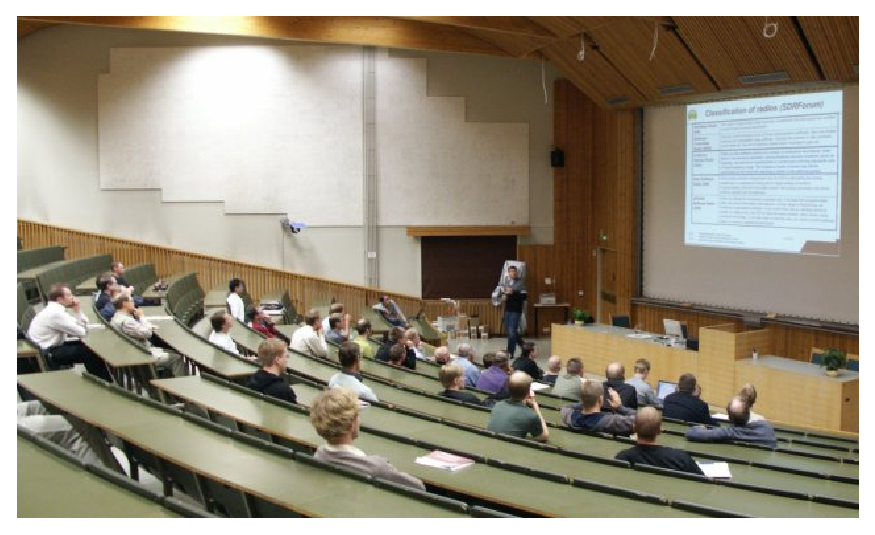
\includegraphics[height=8cm]{kuva2}
% \end{center}
% \caption{Kuvateksti, jossa on liitteen numerointi}
% \label{liitekuva}
% \end{figure}
% %%
% Liitteiden taulukoiden numerointi on kuvien ja kaavojen kaltainen:
% \begin{table}[htb]
% \caption{Taulukon kuvateksti.}
% \label{liitetaulukko}
% \begin{center}
% \fbox{
% \begin{tabular}{lp{0.5\linewidth}}
% 9.00--9.55  & K\"aytett\"avyystestauksen tiedotustilaisuus (osanottajat
% ovat saaneet s\"ahk\"opostitse valmistautumisteht\"av\"at, joten tiedotustilaisuus
% voidaan pit\"a\"a lyhyen\"a).\\
% 9.55--10.00 & Testausalueelle siirtyminen
% \end{tabular}}
% \end{center}
% \end{table}
% Kaavojen numerointi muodostaa liitteiss\"a oman kokonaisuutensa:
% \begin{eqnarray}
% T_{ik} &=& -p g_{ik} + w u_i u_k + \tau_{ik},  \label{liitekaava3} \\
% n_i    &=& n u_i + v_i.                      \label{liitekaava4}
% \end{eqnarray}
% 
\end{document}
% 